\section{Full-Test Detection Benchmark}
\label{sec:benchmark}
\subsection{Comparison and Results}
The benchmark evaluates the same pretrained student twice. In \emph{own scan
only}, a vehicle's prediction uses only its local observation and sharing is
disabled. In \emph{cooperative perception}, the student also uses aligned
features from the other active vehicles. Holding weights fixed isolates the
effect of enabling collaboration in this model. It does not compare two
separately trained detectors, and own scan only is not the paper's separately
trained lower-bound baseline.

Table~\ref{tab:full-test} contains the complete-split results from the saved
benchmark. Cooperation raises AP by
\ReportGainFifty\ percentage points at IoU 0.5 and \ReportGainSeventy\ points
at IoU 0.7. Improvements at both thresholds show that the gain is not
restricted to lenient box overlap in this evaluation.

\begin{table}[htbp]
\centering
\caption{Detection AP on 1,000 test frames and 4,000 active vehicle views.
Both conditions use the same epoch-100 weights.}
\label{tab:full-test}
\input{full-test-table.generated}
\end{table}

\begin{figure}[htbp]
\centering
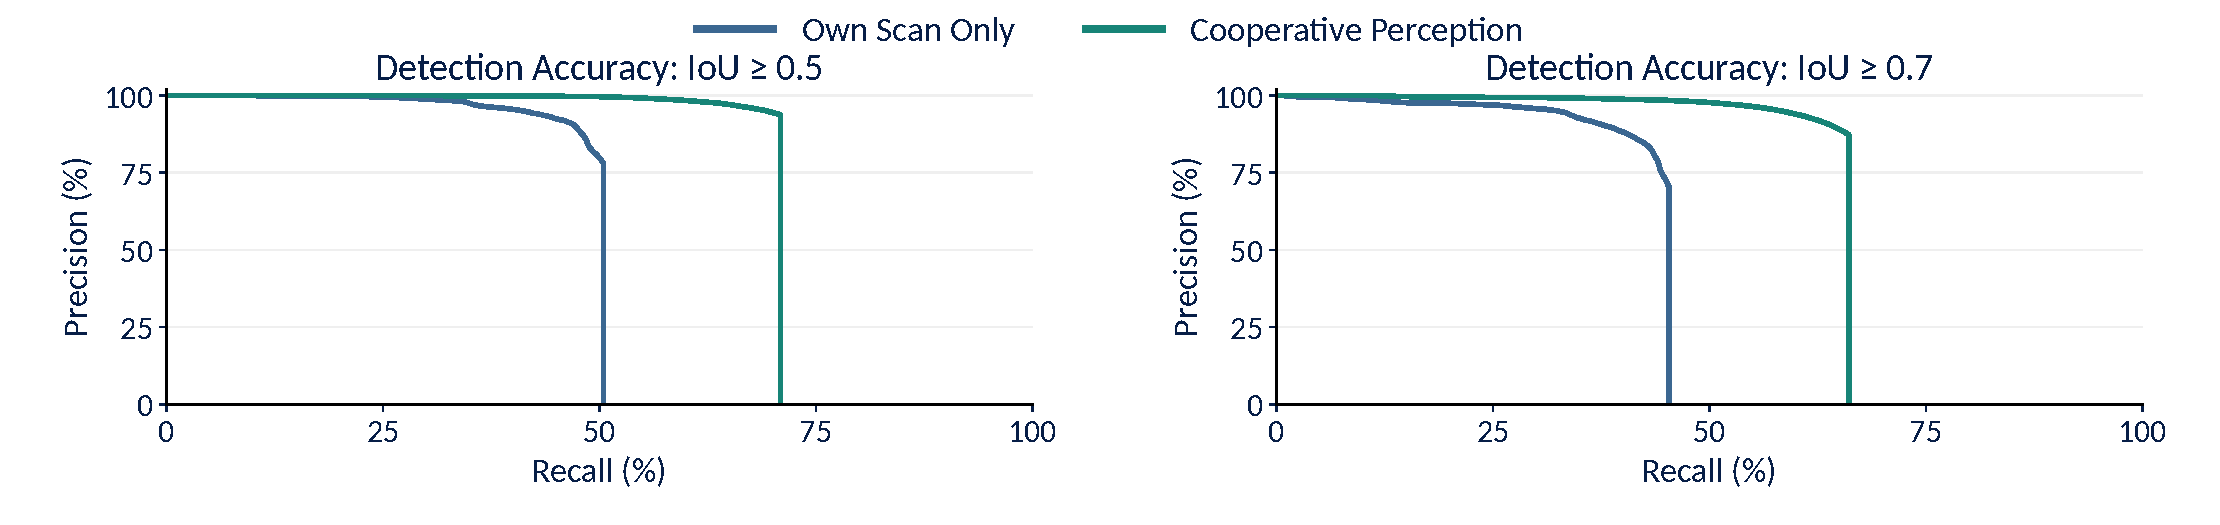
\includegraphics[width=\linewidth]{experiments/w45-2026-11-04/results-plots-v1.pdf}
\caption[Recorded full-test precision--recall curves]{Recorded full-test
precision--recall curves at IoU 0.5 and 0.7.
The curves and plotted values are reused from the saved evaluation, without
new inference or redrawing of the measured data.}
\label{fig:pr}
\end{figure}

The reproduced cooperative scores are approximately 70.4120\% and
64.8237\%. The archived audit compares these with the maintainer's checkpoint
log, 70.4136\% and 64.8239\%, respectively; the discrepancies are below
0.002 percentage points. The documentation table instead lists 69.03\% and
63.44\%. Agreement with the checkpoint log should not be described as
agreement with every published reference table, nor as replication of the
original paper's different-release benchmark.

The saved all-active-view accounting and the authors' collection policy give
identical AP and omit no active views. The record also reports exact
self-only output parity and selected postprocessing parity checks. These
checks support the implementation comparison, but do not establish robustness
to other datasets, checkpoints, or communication conditions.

\subsection{Fixed-Checkpoint Test Loss}
The supplementary record reports classification, box-localization, and total
test loss. Table~\ref{tab:loss} gives the unrounded-source
values displayed to two decimals. The original test code sums loss across
five padded vehicle slots, divides by five, and then averages across
synchronized frames. Inactive slots contribute zero. Thus these values
must be interpreted with that normalization rather than as loss per active
vehicle or a count of incorrect detections.

\begin{table}[htbp]
\centering
\caption{Mean fixed-checkpoint test loss under the authors' normalization.
No teacher or distillation term is included during evaluation.}
\label{tab:loss}
\input{loss-table.generated}
\end{table}

All three loss values are lower with collaboration, consistent with the AP
comparison. This is one evaluation of a fixed checkpoint, not a training
curve, learning-speed comparison, or reconstruction of validation history.
The loss and AP records therefore answer related but different questions.

\subsection{Qualitative Detection Example}
Figure~\ref{fig:detections} shows ego vehicle 1 in raw \texttt{scene\_5},
frame \texttt{000066}, with five participating vehicles. This example comes
from the recorded validation scene, not the 1,000-frame test benchmark.
Within the ego crop, there are 17 reference car boxes. Own scan only produces
11 predictions, while cooperation produces 17. At IoU at least 0.5, the
predictions match 10 and 16 reference cars, respectively.
Equal prediction and reference counts in the cooperative
case therefore do not mean perfect matching.

\begin{figure}[htbp]
\centering
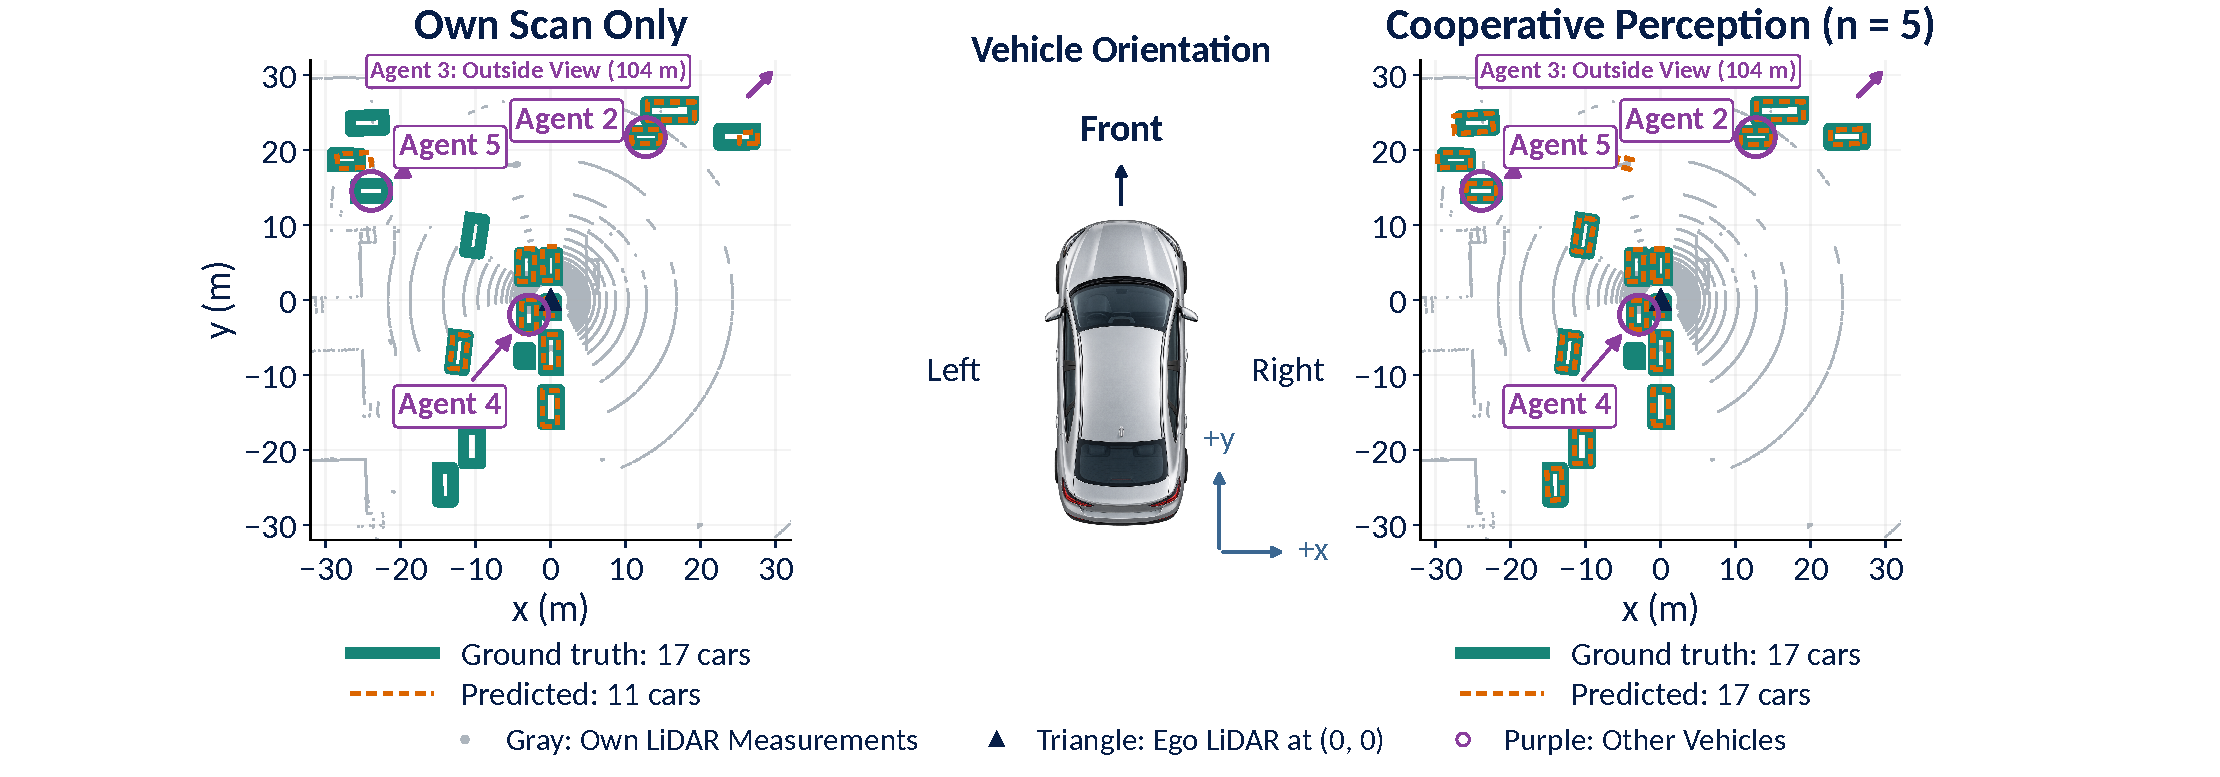
\includegraphics[width=\linewidth]{experiments/w45-2026-11-04/example-detections-v1.pdf}
\caption[Recorded local and cooperative car detections]{Recorded local and cooperative car detections in the single-frame
example. Reference and prediction outlines remain overlaid. Axes use the
vehicle-relative front-up display about the LiDAR sensor; the original
model coordinates are unchanged. The orientation icon is illustrative AI
artwork; points, reference boxes, and predictions are recorded data.}
\label{fig:detections}
\end{figure}

The example illustrates why sharing can help: another viewpoint can supply
useful features where the receiver's own observation is incomplete.
Its counts do not measure full-test AP or the performance of all five
receivers. The camera views in the slide appendix provide synchronized
context, but camera and LiDAR positions differ and the model does not use
those images as detector inputs.

\begin{figure}[htbp]
\centering
\begin{minipage}[t]{0.32\linewidth}
\centering\small\textbf{Front left}\par\smallskip
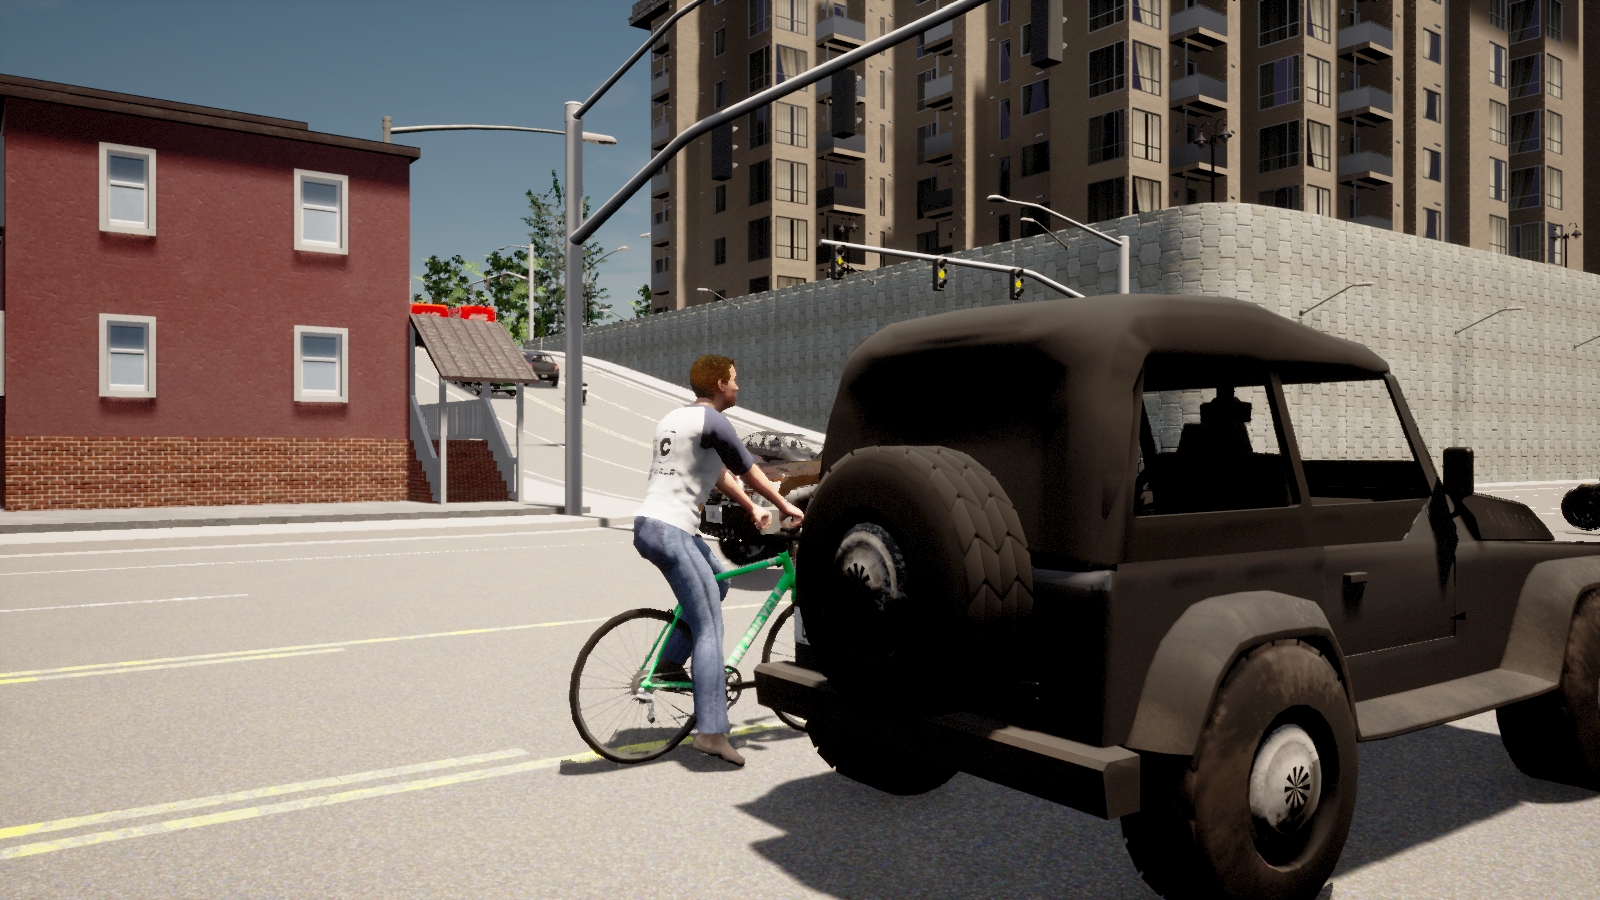
\includegraphics[width=\linewidth]{cameras/example-camera-front-left-v1.jpg}
\end{minipage}\hfill
\begin{minipage}[t]{0.32\linewidth}
\centering\small\textbf{Front}\par\smallskip
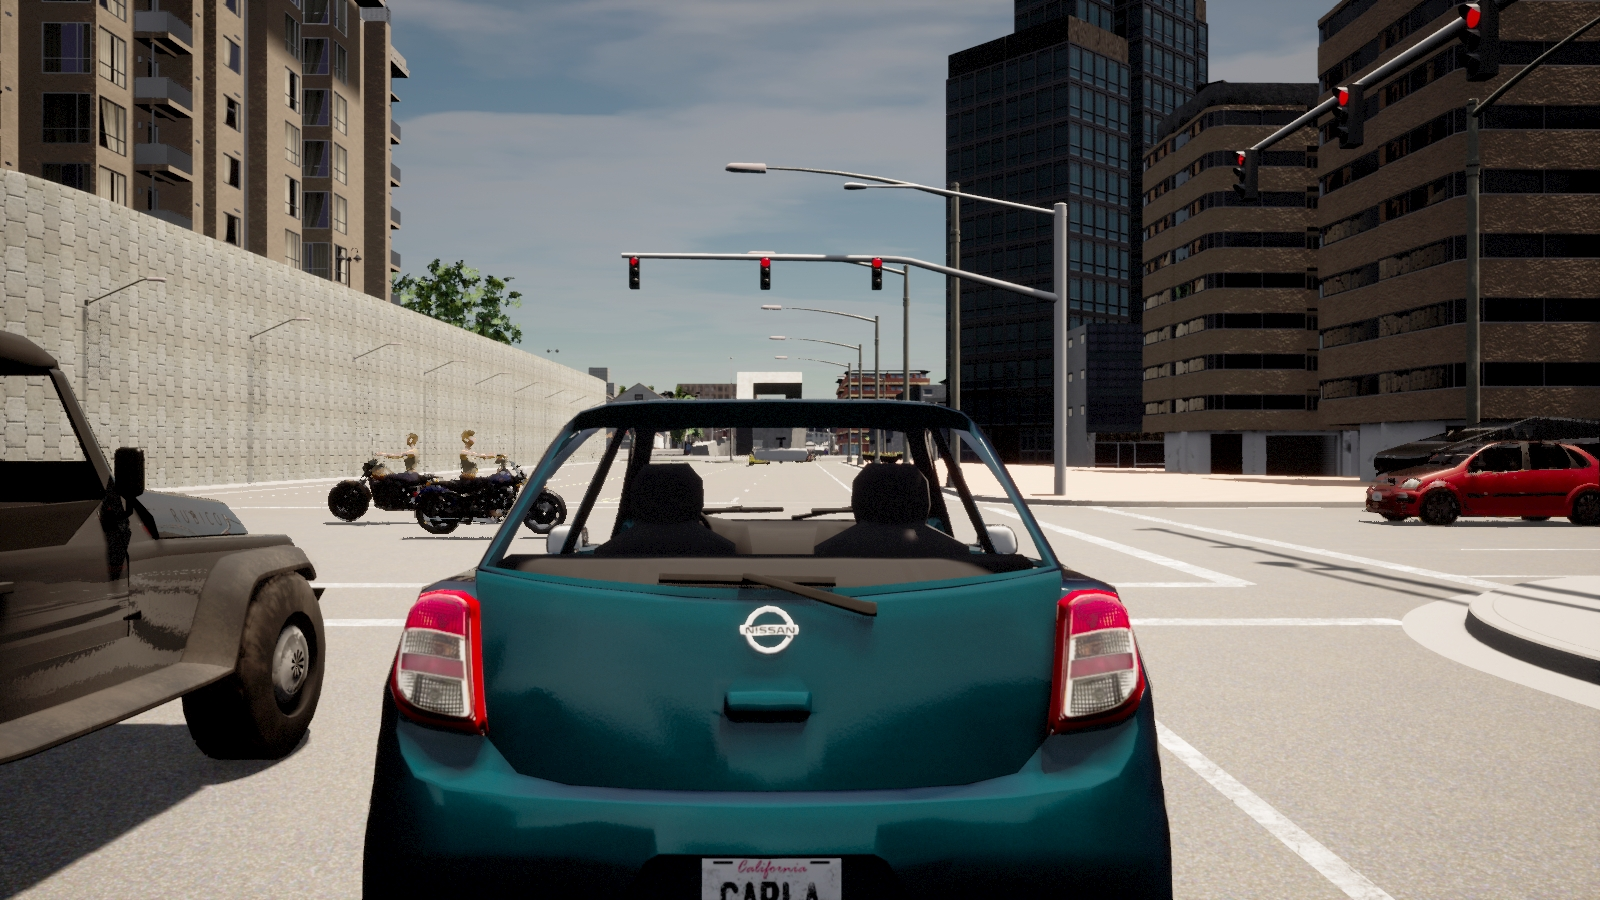
\includegraphics[width=\linewidth]{cameras/example-camera-front-v1.jpg}
\end{minipage}\hfill
\begin{minipage}[t]{0.32\linewidth}
\centering\small\textbf{Front right}\par\smallskip
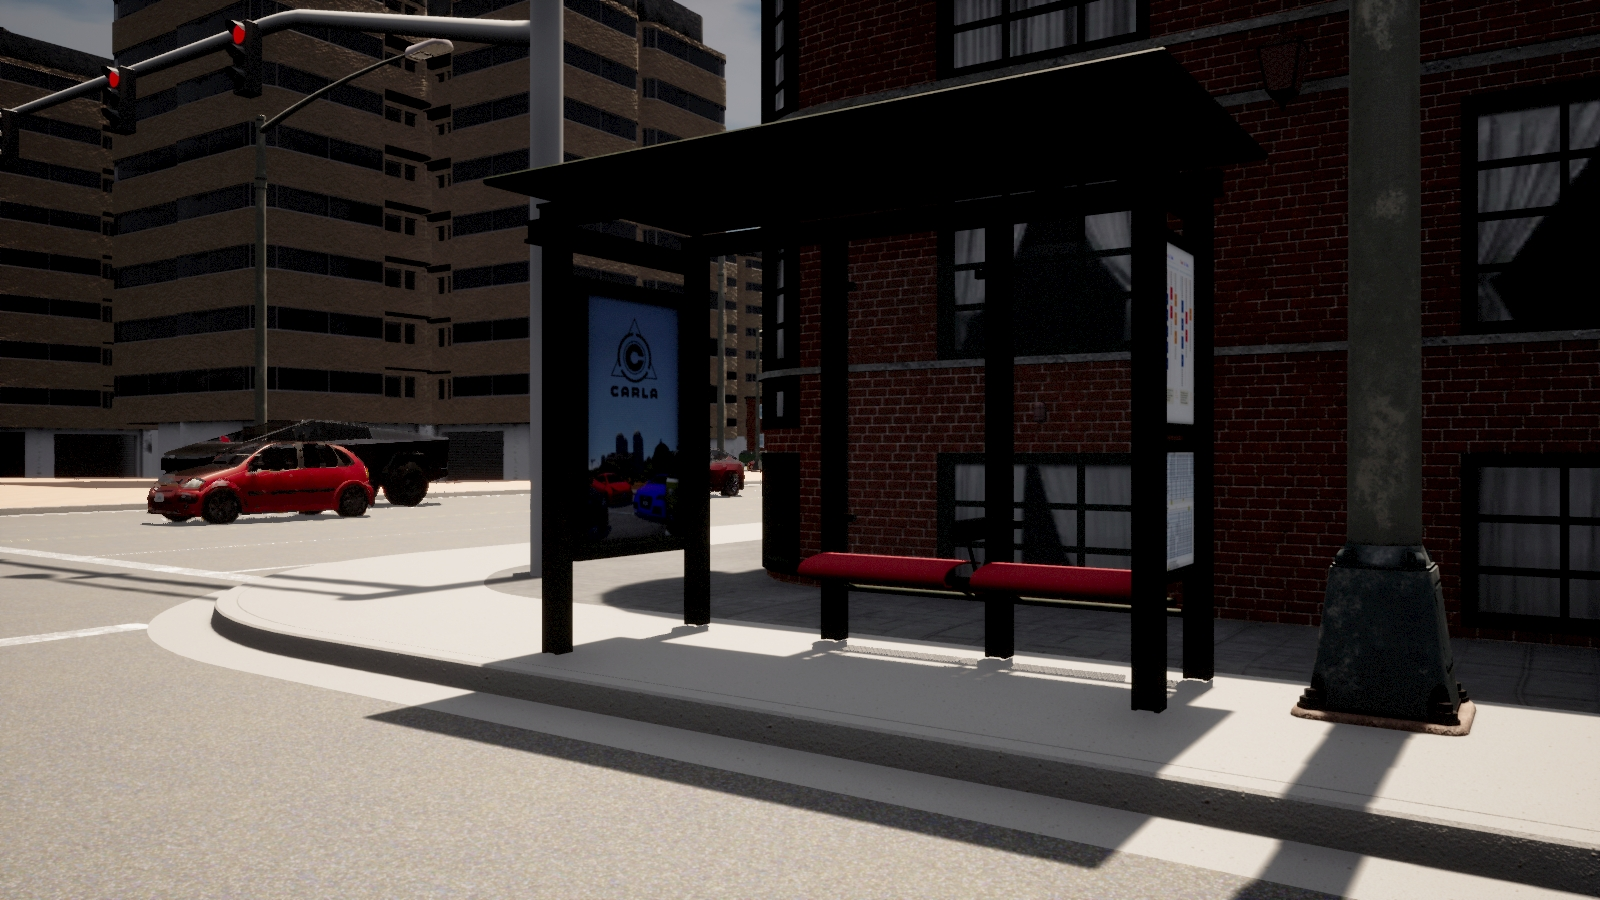
\includegraphics[width=\linewidth]{cameras/example-camera-front-right-v1.jpg}
\end{minipage}\par\medskip
\begin{minipage}[t]{0.32\linewidth}
\centering\small\textbf{Rear left}\par\smallskip
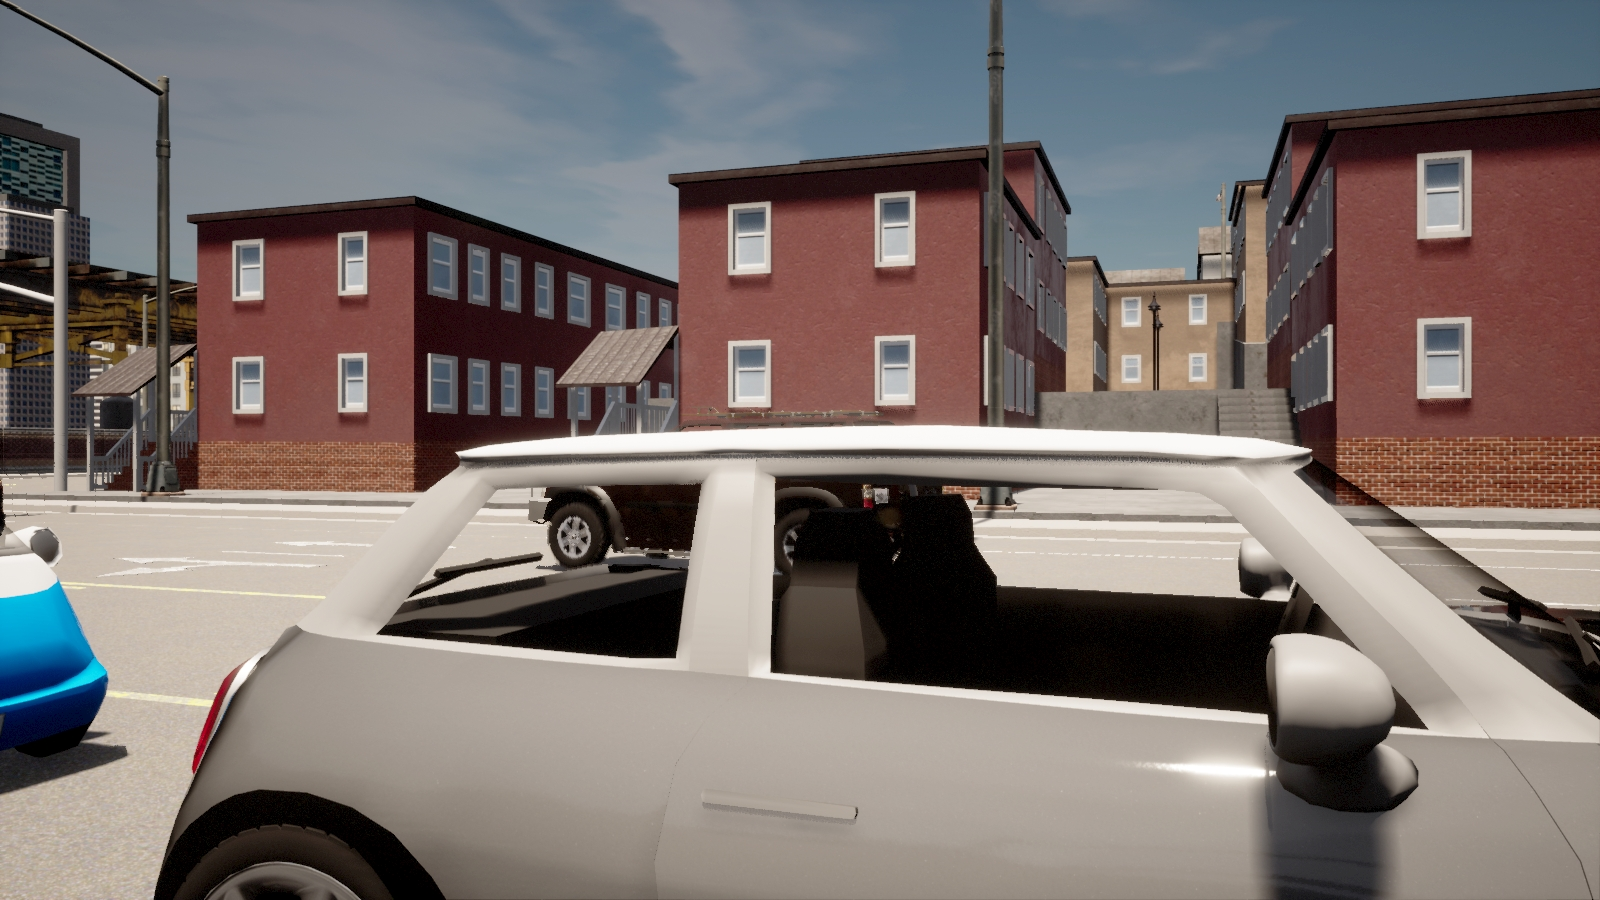
\includegraphics[width=\linewidth]{cameras/example-camera-back-left-v1.jpg}
\end{minipage}\hfill
\begin{minipage}[t]{0.32\linewidth}
\centering\small\textbf{Rear}\par\smallskip
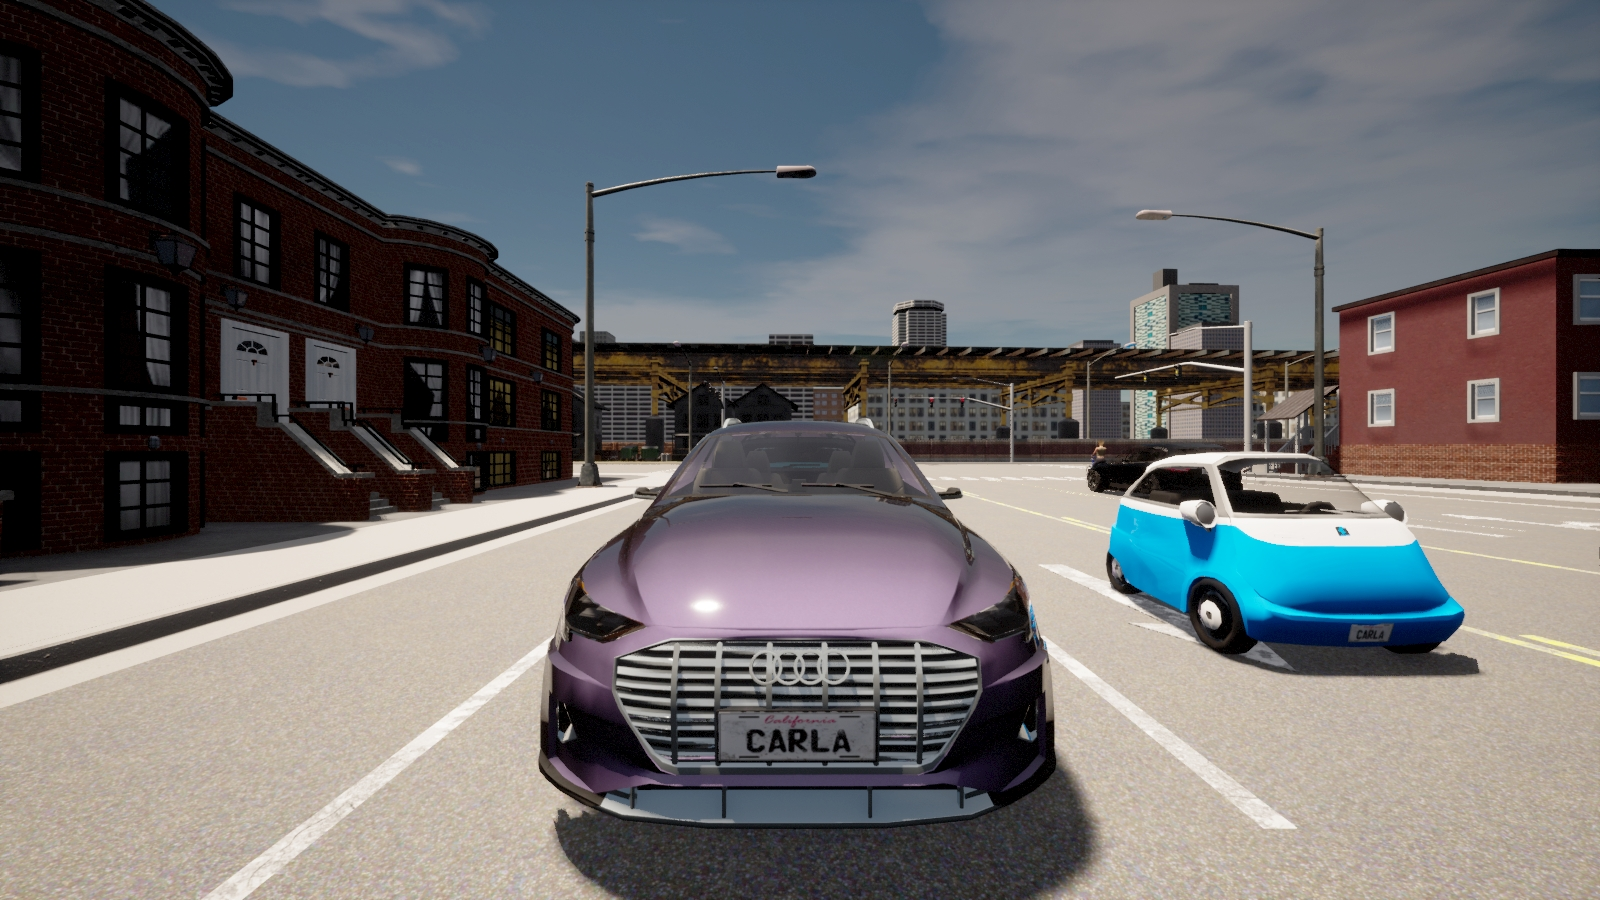
\includegraphics[width=\linewidth]{cameras/example-camera-back-v1.jpg}
\end{minipage}\hfill
\begin{minipage}[t]{0.32\linewidth}
\centering\small\textbf{Rear right}\par\smallskip
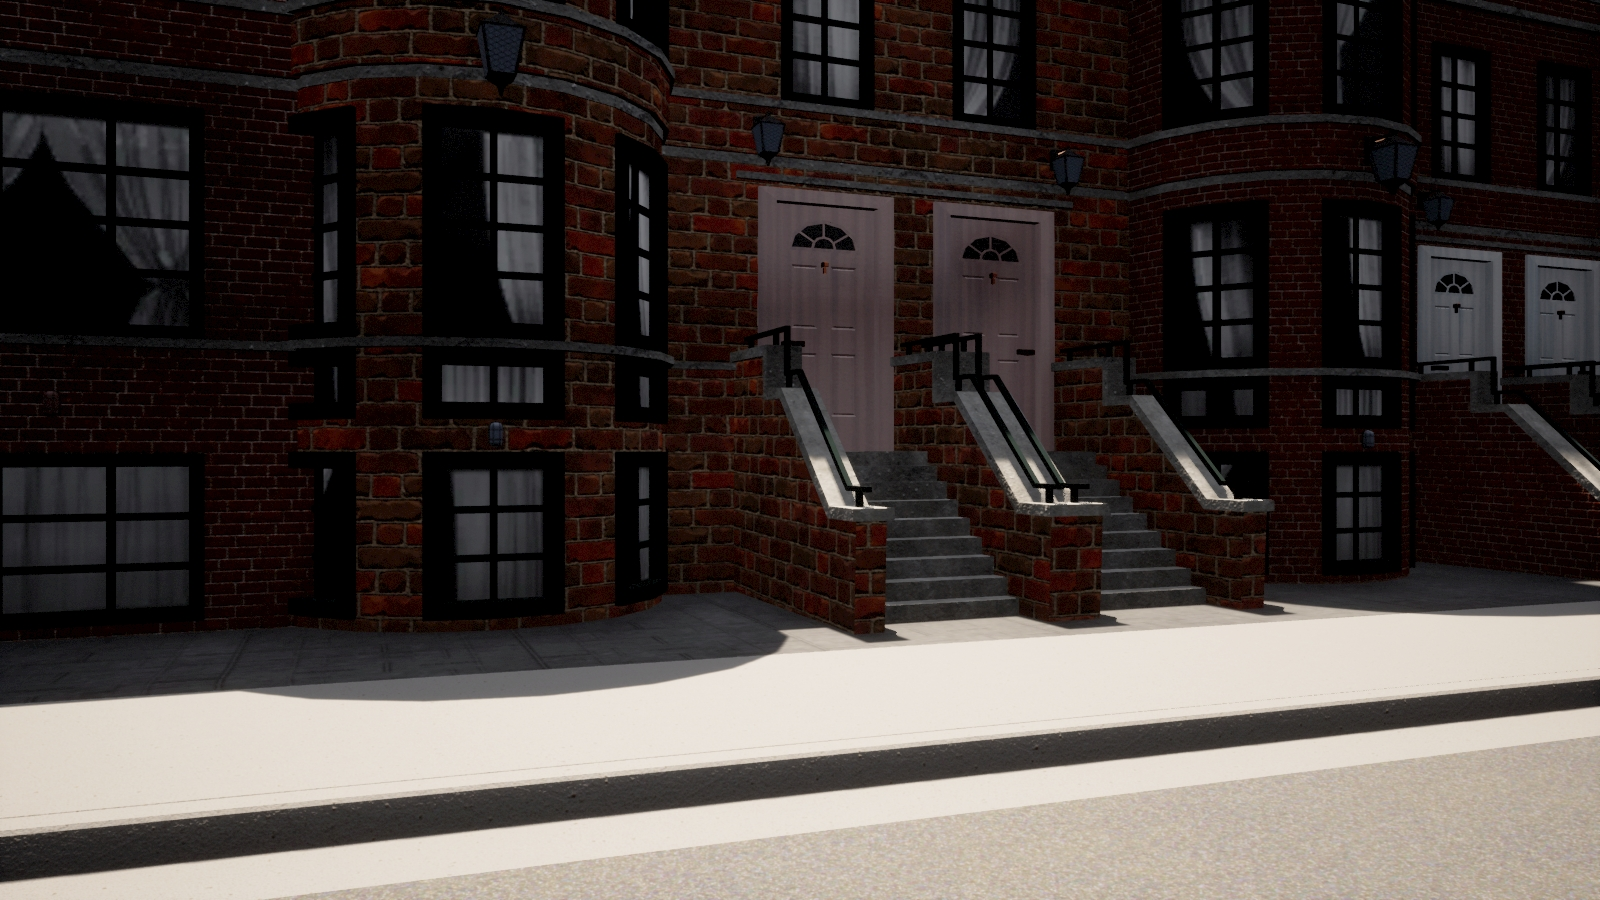
\includegraphics[width=\linewidth]{cameras/example-camera-back-right-v1.jpg}
\end{minipage}
\caption[Six synchronized camera views of the detection example]{The six
V2X-Sim 2.0 camera views archived with the project's \texttt{scene\_5},
frame \texttt{000066} example. They show the surrounding road geometry and
traffic from the ego vehicle.}
\label{fig:example-cameras}
\end{figure}

Figure~\ref{fig:example-cameras} provides the visual setting for the
bird's-eye detection overlays. The views explain why a nearby vehicle and
a farther reference box can have different visibility from the ego sensor.
They also show why the reference-box set should not be equated with the
returns visible in one scan. Camera and LiDAR mounting positions differ,
so the camera panels supply scene context rather than a pixel-level
projection of every LiDAR point.

The useful comparison in Figure~\ref{fig:detections} is therefore which
reference boxes gain a sufficiently overlapping prediction when sharing
is enabled, rather than whether the scene looks busier or the output
contains more boxes. The 10-to-16 increase in matched references supports
that interpretation for this example. Aggregate AP is still determined by
the full ranked evaluation, including false positives and missed references.
